% Options for packages loaded elsewhere
\PassOptionsToPackage{unicode}{hyperref}
\PassOptionsToPackage{hyphens}{url}
%
\documentclass[
]{article}
\usepackage{amsmath,amssymb}
\usepackage{lmodern}
\usepackage{iftex}
\ifPDFTeX
  \usepackage[T1]{fontenc}
  \usepackage[utf8]{inputenc}
  \usepackage{textcomp} % provide euro and other symbols
\else % if luatex or xetex
  \usepackage{unicode-math}
  \defaultfontfeatures{Scale=MatchLowercase}
  \defaultfontfeatures[\rmfamily]{Ligatures=TeX,Scale=1}
\fi
% Use upquote if available, for straight quotes in verbatim environments
\IfFileExists{upquote.sty}{\usepackage{upquote}}{}
\IfFileExists{microtype.sty}{% use microtype if available
  \usepackage[]{microtype}
  \UseMicrotypeSet[protrusion]{basicmath} % disable protrusion for tt fonts
}{}
\makeatletter
\@ifundefined{KOMAClassName}{% if non-KOMA class
  \IfFileExists{parskip.sty}{%
    \usepackage{parskip}
  }{% else
    \setlength{\parindent}{0pt}
    \setlength{\parskip}{6pt plus 2pt minus 1pt}}
}{% if KOMA class
  \KOMAoptions{parskip=half}}
\makeatother
\usepackage{xcolor}
\IfFileExists{xurl.sty}{\usepackage{xurl}}{} % add URL line breaks if available
\IfFileExists{bookmark.sty}{\usepackage{bookmark}}{\usepackage{hyperref}}
\hypersetup{
  pdftitle={Capstone Bike Sharing},
  pdfauthor={Kangjun Zou},
  hidelinks,
  pdfcreator={LaTeX via pandoc}}
\urlstyle{same} % disable monospaced font for URLs
\usepackage[margin=1in]{geometry}
\usepackage{color}
\usepackage{fancyvrb}
\newcommand{\VerbBar}{|}
\newcommand{\VERB}{\Verb[commandchars=\\\{\}]}
\DefineVerbatimEnvironment{Highlighting}{Verbatim}{commandchars=\\\{\}}
% Add ',fontsize=\small' for more characters per line
\usepackage{framed}
\definecolor{shadecolor}{RGB}{248,248,248}
\newenvironment{Shaded}{\begin{snugshade}}{\end{snugshade}}
\newcommand{\AlertTok}[1]{\textcolor[rgb]{0.94,0.16,0.16}{#1}}
\newcommand{\AnnotationTok}[1]{\textcolor[rgb]{0.56,0.35,0.01}{\textbf{\textit{#1}}}}
\newcommand{\AttributeTok}[1]{\textcolor[rgb]{0.77,0.63,0.00}{#1}}
\newcommand{\BaseNTok}[1]{\textcolor[rgb]{0.00,0.00,0.81}{#1}}
\newcommand{\BuiltInTok}[1]{#1}
\newcommand{\CharTok}[1]{\textcolor[rgb]{0.31,0.60,0.02}{#1}}
\newcommand{\CommentTok}[1]{\textcolor[rgb]{0.56,0.35,0.01}{\textit{#1}}}
\newcommand{\CommentVarTok}[1]{\textcolor[rgb]{0.56,0.35,0.01}{\textbf{\textit{#1}}}}
\newcommand{\ConstantTok}[1]{\textcolor[rgb]{0.00,0.00,0.00}{#1}}
\newcommand{\ControlFlowTok}[1]{\textcolor[rgb]{0.13,0.29,0.53}{\textbf{#1}}}
\newcommand{\DataTypeTok}[1]{\textcolor[rgb]{0.13,0.29,0.53}{#1}}
\newcommand{\DecValTok}[1]{\textcolor[rgb]{0.00,0.00,0.81}{#1}}
\newcommand{\DocumentationTok}[1]{\textcolor[rgb]{0.56,0.35,0.01}{\textbf{\textit{#1}}}}
\newcommand{\ErrorTok}[1]{\textcolor[rgb]{0.64,0.00,0.00}{\textbf{#1}}}
\newcommand{\ExtensionTok}[1]{#1}
\newcommand{\FloatTok}[1]{\textcolor[rgb]{0.00,0.00,0.81}{#1}}
\newcommand{\FunctionTok}[1]{\textcolor[rgb]{0.00,0.00,0.00}{#1}}
\newcommand{\ImportTok}[1]{#1}
\newcommand{\InformationTok}[1]{\textcolor[rgb]{0.56,0.35,0.01}{\textbf{\textit{#1}}}}
\newcommand{\KeywordTok}[1]{\textcolor[rgb]{0.13,0.29,0.53}{\textbf{#1}}}
\newcommand{\NormalTok}[1]{#1}
\newcommand{\OperatorTok}[1]{\textcolor[rgb]{0.81,0.36,0.00}{\textbf{#1}}}
\newcommand{\OtherTok}[1]{\textcolor[rgb]{0.56,0.35,0.01}{#1}}
\newcommand{\PreprocessorTok}[1]{\textcolor[rgb]{0.56,0.35,0.01}{\textit{#1}}}
\newcommand{\RegionMarkerTok}[1]{#1}
\newcommand{\SpecialCharTok}[1]{\textcolor[rgb]{0.00,0.00,0.00}{#1}}
\newcommand{\SpecialStringTok}[1]{\textcolor[rgb]{0.31,0.60,0.02}{#1}}
\newcommand{\StringTok}[1]{\textcolor[rgb]{0.31,0.60,0.02}{#1}}
\newcommand{\VariableTok}[1]{\textcolor[rgb]{0.00,0.00,0.00}{#1}}
\newcommand{\VerbatimStringTok}[1]{\textcolor[rgb]{0.31,0.60,0.02}{#1}}
\newcommand{\WarningTok}[1]{\textcolor[rgb]{0.56,0.35,0.01}{\textbf{\textit{#1}}}}
\usepackage{graphicx}
\makeatletter
\def\maxwidth{\ifdim\Gin@nat@width>\linewidth\linewidth\else\Gin@nat@width\fi}
\def\maxheight{\ifdim\Gin@nat@height>\textheight\textheight\else\Gin@nat@height\fi}
\makeatother
% Scale images if necessary, so that they will not overflow the page
% margins by default, and it is still possible to overwrite the defaults
% using explicit options in \includegraphics[width, height, ...]{}
\setkeys{Gin}{width=\maxwidth,height=\maxheight,keepaspectratio}
% Set default figure placement to htbp
\makeatletter
\def\fps@figure{htbp}
\makeatother
\setlength{\emergencystretch}{3em} % prevent overfull lines
\providecommand{\tightlist}{%
  \setlength{\itemsep}{0pt}\setlength{\parskip}{0pt}}
\setcounter{secnumdepth}{-\maxdimen} % remove section numbering
\ifLuaTeX
  \usepackage{selnolig}  % disable illegal ligatures
\fi

\title{Capstone Bike Sharing}
\author{Kangjun Zou}
\date{2022-05-05}

\begin{document}
\maketitle

\hypertarget{a-statement-of-the-business-task}{%
\subsection{A statement of the business
task}\label{a-statement-of-the-business-task}}

The end goal of this project is to provide insights through data
analysis to assist all stakeholders (Lily Moreno, Cyclistic marketing
team and Cyclistic executive team) to design marketing strategies aimed
at converting casual riders to annual members.

To do that,three questions need to be addresses: 1. How do annual
members and casual riders use Cyclistic bikes differently? 2. Why would
casual riders buy Cyclistic annual memberships? 3. How can Cyclistic use
digital media to influence casual riders to become members?

This project is conducted to answer \emph{the first question only} and
provide a report with the following deliverable: 1. A clear statement of
the business task 2 . A description of all data sources used 3.
Documentations of any cleaning and manipulation of data 4. A summary of
the analysis 5. Supporting visualizations and key findings 6. Top three
3 recommendations based on analysis

\hypertarget{a-description-of-all-the-data-sources-used}{%
\subsection{A description of all the data sources
used}\label{a-description-of-all-the-data-sources-used}}

For this project, we will use the previous 12 months (from 2021-04 to
2022-03) of Cyclistic's historical trip data, provided by Motivate
International Inc, under this \href{www.divvybikes.com}{license}) to
analyze and identify trends.

\hypertarget{documentation-of-any-data-cleaning-or-manipulation-of-data}{%
\subsection{Documentation of any data cleaning or manipulation of
data}\label{documentation-of-any-data-cleaning-or-manipulation-of-data}}

\hypertarget{import-data-from-2021-04-to-2022-03}{%
\subsubsection{--Import data from 2021-04 to
2022-03}\label{import-data-from-2021-04-to-2022-03}}

\begin{Shaded}
\begin{Highlighting}[]
\FunctionTok{library}\NormalTok{(readr)}
\NormalTok{X202104\_trip\_data }\OtherTok{\textless{}{-}} \FunctionTok{read\_csv}\NormalTok{(}\StringTok{"202104\_trip\_data.csv"}\NormalTok{)}
\end{Highlighting}
\end{Shaded}

\begin{verbatim}
## Rows: 337230 Columns: 13
## -- Column specification --------------------------------------------------------
## Delimiter: ","
## chr  (7): ride_id, rideable_type, start_station_name, start_station_id, end_...
## dbl  (4): start_lat, start_lng, end_lat, end_lng
## dttm (2): started_at, ended_at
## 
## i Use `spec()` to retrieve the full column specification for this data.
## i Specify the column types or set `show_col_types = FALSE` to quiet this message.
\end{verbatim}

\begin{Shaded}
\begin{Highlighting}[]
\FunctionTok{View}\NormalTok{(X202104\_trip\_data)}
\FunctionTok{library}\NormalTok{(readr)}
\NormalTok{X202105\_trip\_data }\OtherTok{\textless{}{-}} \FunctionTok{read\_csv}\NormalTok{(}\StringTok{"202105\_trip\_data.csv"}\NormalTok{)}
\end{Highlighting}
\end{Shaded}

\begin{verbatim}
## Rows: 531633 Columns: 13
## -- Column specification --------------------------------------------------------
## Delimiter: ","
## chr  (7): ride_id, rideable_type, start_station_name, start_station_id, end_...
## dbl  (4): start_lat, start_lng, end_lat, end_lng
## dttm (2): started_at, ended_at
## 
## i Use `spec()` to retrieve the full column specification for this data.
## i Specify the column types or set `show_col_types = FALSE` to quiet this message.
\end{verbatim}

\begin{Shaded}
\begin{Highlighting}[]
\FunctionTok{View}\NormalTok{(X202105\_trip\_data)}
\FunctionTok{library}\NormalTok{(readr)}
\NormalTok{X202106\_trip\_data }\OtherTok{\textless{}{-}} \FunctionTok{read\_csv}\NormalTok{(}\StringTok{"202106\_trip\_data.csv"}\NormalTok{)}
\end{Highlighting}
\end{Shaded}

\begin{verbatim}
## Rows: 729595 Columns: 13
## -- Column specification --------------------------------------------------------
## Delimiter: ","
## chr  (7): ride_id, rideable_type, start_station_name, start_station_id, end_...
## dbl  (4): start_lat, start_lng, end_lat, end_lng
## dttm (2): started_at, ended_at
## 
## i Use `spec()` to retrieve the full column specification for this data.
## i Specify the column types or set `show_col_types = FALSE` to quiet this message.
\end{verbatim}

\begin{Shaded}
\begin{Highlighting}[]
\FunctionTok{View}\NormalTok{(X202106\_trip\_data)}
\FunctionTok{library}\NormalTok{(readr)}
\NormalTok{X202107\_trip\_data }\OtherTok{\textless{}{-}} \FunctionTok{read\_csv}\NormalTok{(}\StringTok{"202107\_trip\_data.csv"}\NormalTok{)}
\end{Highlighting}
\end{Shaded}

\begin{verbatim}
## Rows: 822410 Columns: 13
## -- Column specification --------------------------------------------------------
## Delimiter: ","
## chr  (7): ride_id, rideable_type, start_station_name, start_station_id, end_...
## dbl  (4): start_lat, start_lng, end_lat, end_lng
## dttm (2): started_at, ended_at
## 
## i Use `spec()` to retrieve the full column specification for this data.
## i Specify the column types or set `show_col_types = FALSE` to quiet this message.
\end{verbatim}

\begin{Shaded}
\begin{Highlighting}[]
\FunctionTok{View}\NormalTok{(X202107\_trip\_data)}
\FunctionTok{library}\NormalTok{(readr)}
\NormalTok{X202108\_trip\_data }\OtherTok{\textless{}{-}} \FunctionTok{read\_csv}\NormalTok{(}\StringTok{"202108\_trip\_data.csv"}\NormalTok{)}
\end{Highlighting}
\end{Shaded}

\begin{verbatim}
## Rows: 804352 Columns: 13
## -- Column specification --------------------------------------------------------
## Delimiter: ","
## chr  (7): ride_id, rideable_type, start_station_name, start_station_id, end_...
## dbl  (4): start_lat, start_lng, end_lat, end_lng
## dttm (2): started_at, ended_at
## 
## i Use `spec()` to retrieve the full column specification for this data.
## i Specify the column types or set `show_col_types = FALSE` to quiet this message.
\end{verbatim}

\begin{Shaded}
\begin{Highlighting}[]
\FunctionTok{View}\NormalTok{(X202108\_trip\_data)}
\FunctionTok{library}\NormalTok{(readr)}
\NormalTok{X202109\_trip\_data }\OtherTok{\textless{}{-}} \FunctionTok{read\_csv}\NormalTok{(}\StringTok{"202109\_trip\_data.csv"}\NormalTok{)}
\end{Highlighting}
\end{Shaded}

\begin{verbatim}
## Rows: 756147 Columns: 13
## -- Column specification --------------------------------------------------------
## Delimiter: ","
## chr  (7): ride_id, rideable_type, start_station_name, start_station_id, end_...
## dbl  (4): start_lat, start_lng, end_lat, end_lng
## dttm (2): started_at, ended_at
## 
## i Use `spec()` to retrieve the full column specification for this data.
## i Specify the column types or set `show_col_types = FALSE` to quiet this message.
\end{verbatim}

\begin{Shaded}
\begin{Highlighting}[]
\FunctionTok{View}\NormalTok{(X202109\_trip\_data)}
\FunctionTok{library}\NormalTok{(readr)}
\NormalTok{X202110\_trip\_data }\OtherTok{\textless{}{-}} \FunctionTok{read\_csv}\NormalTok{(}\StringTok{"202110\_trip\_data.csv"}\NormalTok{)}
\end{Highlighting}
\end{Shaded}

\begin{verbatim}
## Rows: 631226 Columns: 13
## -- Column specification --------------------------------------------------------
## Delimiter: ","
## chr  (7): ride_id, rideable_type, start_station_name, start_station_id, end_...
## dbl  (4): start_lat, start_lng, end_lat, end_lng
## dttm (2): started_at, ended_at
## 
## i Use `spec()` to retrieve the full column specification for this data.
## i Specify the column types or set `show_col_types = FALSE` to quiet this message.
\end{verbatim}

\begin{Shaded}
\begin{Highlighting}[]
\FunctionTok{View}\NormalTok{(X202110\_trip\_data)}
\FunctionTok{library}\NormalTok{(readr)}
\NormalTok{X202111\_trip\_data }\OtherTok{\textless{}{-}} \FunctionTok{read\_csv}\NormalTok{(}\StringTok{"202111\_trip\_data.csv"}\NormalTok{)}
\end{Highlighting}
\end{Shaded}

\begin{verbatim}
## Rows: 359978 Columns: 13
## -- Column specification --------------------------------------------------------
## Delimiter: ","
## chr  (7): ride_id, rideable_type, start_station_name, start_station_id, end_...
## dbl  (4): start_lat, start_lng, end_lat, end_lng
## dttm (2): started_at, ended_at
## 
## i Use `spec()` to retrieve the full column specification for this data.
## i Specify the column types or set `show_col_types = FALSE` to quiet this message.
\end{verbatim}

\begin{Shaded}
\begin{Highlighting}[]
\FunctionTok{View}\NormalTok{(X202111\_trip\_data)}
\FunctionTok{library}\NormalTok{(readr)}
\NormalTok{X202112\_trip\_data }\OtherTok{\textless{}{-}} \FunctionTok{read\_csv}\NormalTok{(}\StringTok{"202112\_trip\_data.csv"}\NormalTok{)}
\end{Highlighting}
\end{Shaded}

\begin{verbatim}
## Rows: 247540 Columns: 13
## -- Column specification --------------------------------------------------------
## Delimiter: ","
## chr  (7): ride_id, rideable_type, start_station_name, start_station_id, end_...
## dbl  (4): start_lat, start_lng, end_lat, end_lng
## dttm (2): started_at, ended_at
## 
## i Use `spec()` to retrieve the full column specification for this data.
## i Specify the column types or set `show_col_types = FALSE` to quiet this message.
\end{verbatim}

\begin{Shaded}
\begin{Highlighting}[]
\FunctionTok{View}\NormalTok{(X202112\_trip\_data)}
\FunctionTok{library}\NormalTok{(readr)}
\NormalTok{X202201\_trip\_data }\OtherTok{\textless{}{-}} \FunctionTok{read\_csv}\NormalTok{(}\StringTok{"202201\_trip\_data.csv"}\NormalTok{)}
\end{Highlighting}
\end{Shaded}

\begin{verbatim}
## Rows: 103770 Columns: 13
## -- Column specification --------------------------------------------------------
## Delimiter: ","
## chr  (7): ride_id, rideable_type, start_station_name, start_station_id, end_...
## dbl  (4): start_lat, start_lng, end_lat, end_lng
## dttm (2): started_at, ended_at
## 
## i Use `spec()` to retrieve the full column specification for this data.
## i Specify the column types or set `show_col_types = FALSE` to quiet this message.
\end{verbatim}

\begin{Shaded}
\begin{Highlighting}[]
\FunctionTok{View}\NormalTok{(X202201\_trip\_data)}
\FunctionTok{library}\NormalTok{(readr)}
\NormalTok{X202202\_trip\_data }\OtherTok{\textless{}{-}} \FunctionTok{read\_csv}\NormalTok{(}\StringTok{"202202\_trip\_data.csv"}\NormalTok{)}
\end{Highlighting}
\end{Shaded}

\begin{verbatim}
## Rows: 115609 Columns: 13
## -- Column specification --------------------------------------------------------
## Delimiter: ","
## chr  (7): ride_id, rideable_type, start_station_name, start_station_id, end_...
## dbl  (4): start_lat, start_lng, end_lat, end_lng
## dttm (2): started_at, ended_at
## 
## i Use `spec()` to retrieve the full column specification for this data.
## i Specify the column types or set `show_col_types = FALSE` to quiet this message.
\end{verbatim}

\begin{Shaded}
\begin{Highlighting}[]
\FunctionTok{View}\NormalTok{(X202201\_trip\_data)}
\FunctionTok{library}\NormalTok{(readr)}
\NormalTok{X202203\_trip\_data }\OtherTok{\textless{}{-}} \FunctionTok{read\_csv}\NormalTok{(}\StringTok{"202203\_trip\_data.csv"}\NormalTok{)}
\end{Highlighting}
\end{Shaded}

\begin{verbatim}
## Rows: 284042 Columns: 13
## -- Column specification --------------------------------------------------------
## Delimiter: ","
## chr  (7): ride_id, rideable_type, start_station_name, start_station_id, end_...
## dbl  (4): start_lat, start_lng, end_lat, end_lng
## dttm (2): started_at, ended_at
## 
## i Use `spec()` to retrieve the full column specification for this data.
## i Specify the column types or set `show_col_types = FALSE` to quiet this message.
\end{verbatim}

\begin{Shaded}
\begin{Highlighting}[]
\FunctionTok{View}\NormalTok{(X202203\_trip\_data)}
\end{Highlighting}
\end{Shaded}

\hypertarget{findings-all-12-data-frames-have-the-same-structure}{%
\paragraph{Findings: All 12 data frames have the same
structure}\label{findings-all-12-data-frames-have-the-same-structure}}

\hypertarget{combine-data-from-2021-04-to-2022-03-for-easier-data-cleaning-and-manipulation}{%
\subsubsection{Combine data from 2021-04 to 2022-03 for easier data
cleaning and
manipulation}\label{combine-data-from-2021-04-to-2022-03-for-easier-data-cleaning-and-manipulation}}

\begin{Shaded}
\begin{Highlighting}[]
\NormalTok{trip\_data\_combined}\OtherTok{\textless{}{-}}\FunctionTok{rbind}\NormalTok{(X202104\_trip\_data,X202105\_trip\_data,X202106\_trip\_data,X202107\_trip\_data,X202108\_trip\_data,X202109\_trip\_data,X202110\_trip\_data,X202111\_trip\_data,X202112\_trip\_data,X202201\_trip\_data,X202202\_trip\_data,X202203\_trip\_data)}
\end{Highlighting}
\end{Shaded}

\hypertarget{findings-notice-lots-of-na}{%
\paragraph{Findings: Notice lots of
``NA''}\label{findings-notice-lots-of-na}}

\hypertarget{drop-na-to-avoid-misleading-data-assuming-entries-with-na-are-not-real-rides-by-users}{%
\subsubsection{Drop ``NA'' to avoid misleading data, assuming entries
with ``NA'' are not real rides by
users}\label{drop-na-to-avoid-misleading-data-assuming-entries-with-na-are-not-real-rides-by-users}}

\begin{Shaded}
\begin{Highlighting}[]
\FunctionTok{library}\NormalTok{(tidyverse)}
\end{Highlighting}
\end{Shaded}

\begin{verbatim}
## -- Attaching packages --------------------------------------- tidyverse 1.3.1 --
\end{verbatim}

\begin{verbatim}
## v ggplot2 3.3.6     v dplyr   1.0.9
## v tibble  3.1.6     v stringr 1.4.0
## v tidyr   1.2.0     v forcats 0.5.1
## v purrr   0.3.4
\end{verbatim}

\begin{verbatim}
## -- Conflicts ------------------------------------------ tidyverse_conflicts() --
## x dplyr::filter() masks stats::filter()
## x dplyr::lag()    masks stats::lag()
\end{verbatim}

\begin{Shaded}
\begin{Highlighting}[]
\NormalTok{trip\_data\_nadrop}\OtherTok{\textless{}{-}}\NormalTok{trip\_data\_combined }\SpecialCharTok{\%\textgreater{}\%} \FunctionTok{drop\_na}\NormalTok{()}
\end{Highlighting}
\end{Shaded}

\hypertarget{add-a-new-column-ride_length-to-calculate-time-intervals-between-started_at-and-ended_at-and-rename-it-as-trip_data_nadrop_ridelength}{%
\subsubsection{Add a new column ``ride\_length'' to calculate time
intervals between ``started\_at'' and ``ended\_at'' and rename it as
``trip\_data\_nadrop\_ridelength''}\label{add-a-new-column-ride_length-to-calculate-time-intervals-between-started_at-and-ended_at-and-rename-it-as-trip_data_nadrop_ridelength}}

\begin{Shaded}
\begin{Highlighting}[]
\NormalTok{x}\OtherTok{\textless{}{-}}\NormalTok{trip\_data\_nadrop}
\NormalTok{x}\SpecialCharTok{$}\NormalTok{ride\_length}\OtherTok{\textless{}{-}}\FunctionTok{difftime}\NormalTok{(trip\_data\_nadrop}\SpecialCharTok{$}\NormalTok{ended\_at,trip\_data\_nadrop}\SpecialCharTok{$}\NormalTok{started\_at)}
\NormalTok{trip\_data\_nadrop\_ridelength}\OtherTok{\textless{}{-}}\NormalTok{x}
\end{Highlighting}
\end{Shaded}

\hypertarget{find-rides-with-ride_length0-further-filtering-requires-investigation-into-the-data-set-with-stakeholders}{%
\subsubsection{Find rides with ``ride\_length''\textless=0, further
filtering requires investigation into the data set with
stakeholders}\label{find-rides-with-ride_length0-further-filtering-requires-investigation-into-the-data-set-with-stakeholders}}

\begin{Shaded}
\begin{Highlighting}[]
\NormalTok{outliers}\OtherTok{\textless{}{-}}\FunctionTok{filter}\NormalTok{(trip\_data\_nadrop\_ridelength,ride\_length}\SpecialCharTok{\textless{}=}\DecValTok{0}\NormalTok{)}
\end{Highlighting}
\end{Shaded}

\hypertarget{findings-there-are-207-rides-with-ride_length0}{%
\paragraph{Findings: There are 207 rides with
``ride\_length''\textless=0}\label{findings-there-are-207-rides-with-ride_length0}}

\hypertarget{filter-out-rides-with-ride_length0}{%
\subsubsection{Filter out rides with
``ride\_length''\textless=0}\label{filter-out-rides-with-ride_length0}}

\begin{Shaded}
\begin{Highlighting}[]
\NormalTok{trip\_data\_nadrop\_ridelength\_nooutliers}\OtherTok{\textless{}{-}}\FunctionTok{filter}\NormalTok{(trip\_data\_nadrop\_ridelength,ride\_length}\SpecialCharTok{\textgreater{}}\DecValTok{0}\NormalTok{)}
\end{Highlighting}
\end{Shaded}

\hypertarget{create-new-columns-weekday-month-quarter-hour}{%
\subsubsection{Create new columns: ``weekday'', ``month'', ``quarter'',
``hour''}\label{create-new-columns-weekday-month-quarter-hour}}

\begin{Shaded}
\begin{Highlighting}[]
\NormalTok{x}\OtherTok{\textless{}{-}}\NormalTok{trip\_data\_nadrop\_ridelength\_nooutliers}
\NormalTok{x}\SpecialCharTok{$}\NormalTok{weekday}\OtherTok{\textless{}{-}}\FunctionTok{weekdays}\NormalTok{(trip\_data\_nadrop\_ridelength\_nooutliers}\SpecialCharTok{$}\NormalTok{started\_at)}
\NormalTok{x}\SpecialCharTok{$}\NormalTok{month}\OtherTok{\textless{}{-}}\FunctionTok{months}\NormalTok{(trip\_data\_nadrop\_ridelength\_nooutliers}\SpecialCharTok{$}\NormalTok{started\_at)}
\NormalTok{x}\SpecialCharTok{$}\NormalTok{quarter}\OtherTok{\textless{}{-}}\FunctionTok{quarters}\NormalTok{(trip\_data\_nadrop\_ridelength\_nooutliers}\SpecialCharTok{$}\NormalTok{started\_at)}
\NormalTok{x}\SpecialCharTok{$}\NormalTok{hour}\OtherTok{\textless{}{-}}\FunctionTok{format}\NormalTok{(trip\_data\_nadrop\_ridelength\_nooutliers}\SpecialCharTok{$}\NormalTok{started\_at,}\StringTok{"\%H"}\NormalTok{)}
\NormalTok{trip\_data\_clean}\OtherTok{\textless{}{-}}\NormalTok{x}
\FunctionTok{remove}\NormalTok{(x)}
\end{Highlighting}
\end{Shaded}

\hypertarget{supporting-visulizations-and-key-findings}{%
\subsection{Supporting visulizations and key
findings}\label{supporting-visulizations-and-key-findings}}

\begin{enumerate}
\def\labelenumi{\arabic{enumi}.}
\tightlist
\item
  Which user type bikes more often?
\end{enumerate}

\begin{Shaded}
\begin{Highlighting}[]
\FunctionTok{ggplot}\NormalTok{(}\AttributeTok{data =}\NormalTok{ trip\_data\_clean)}\SpecialCharTok{+}\FunctionTok{geom\_bar}\NormalTok{(}\AttributeTok{mapping =} \FunctionTok{aes}\NormalTok{(}\AttributeTok{x=}\NormalTok{member\_casual,}\AttributeTok{fill=}\NormalTok{member\_casual))}\SpecialCharTok{+}\FunctionTok{labs}\NormalTok{(}\AttributeTok{title=}\NormalTok{(}\StringTok{"Which user type bikes more often?"}\NormalTok{),}\AttributeTok{subtitle =}\StringTok{"Casual vs Member from 2021{-}04 to 2022{-}03"}\NormalTok{, }\AttributeTok{x=}\StringTok{"User type"}\NormalTok{, }\AttributeTok{y=}\StringTok{"Number of rides"}\NormalTok{,}\AttributeTok{caption =} \StringTok{"1e+06=1,000,000, Data provided by Motivate International Inc."}\NormalTok{)}\SpecialCharTok{+}\FunctionTok{scale\_fill\_discrete}\NormalTok{(}\AttributeTok{name=}\StringTok{"User type"}\NormalTok{)}
\end{Highlighting}
\end{Shaded}

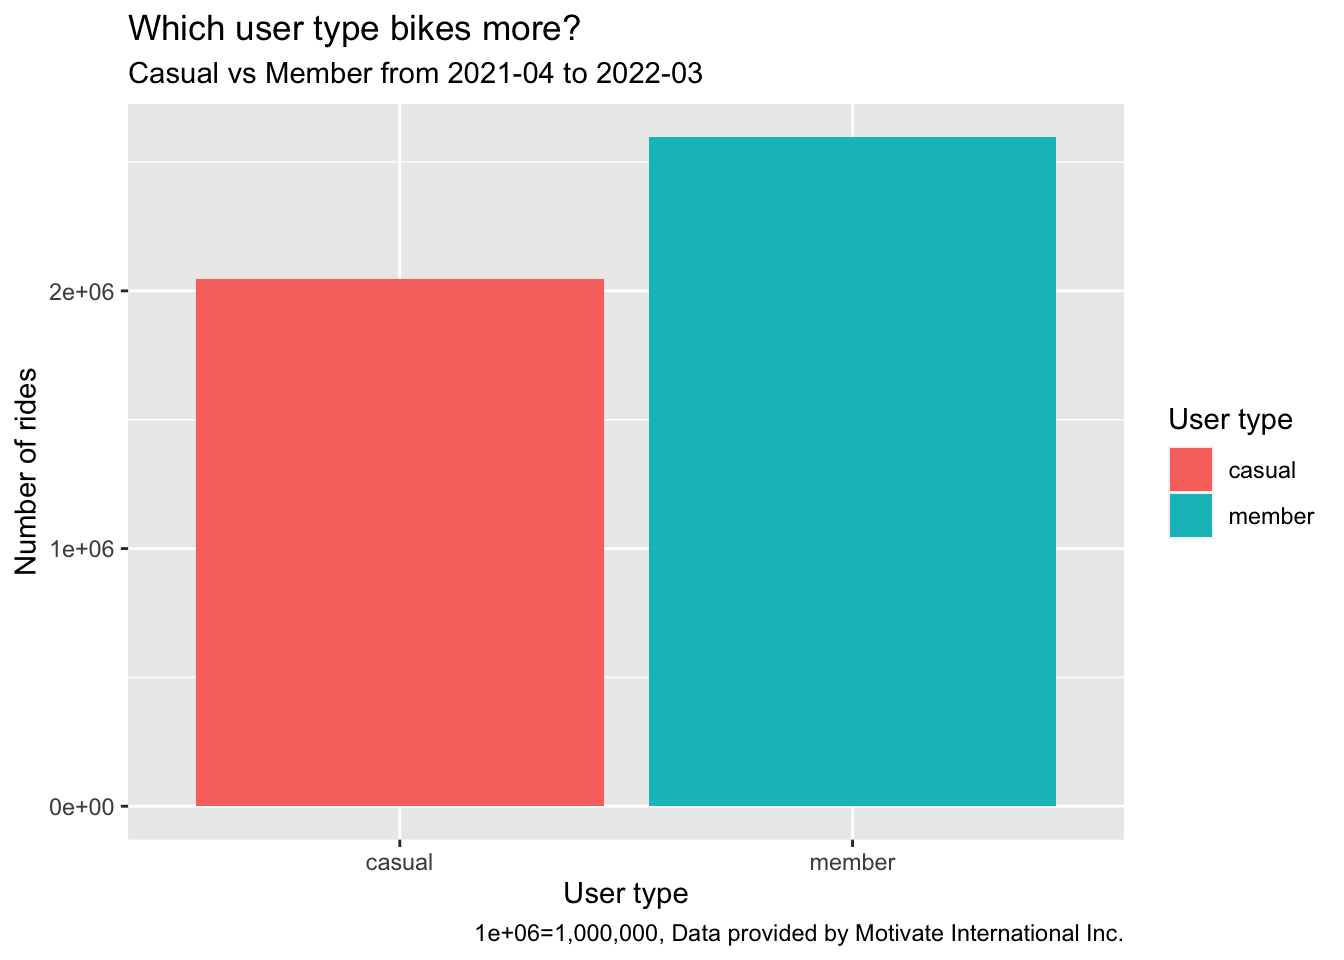
\includegraphics{capstone_bike_sharing_v02_files/figure-latex/unnamed-chunk-8-1.pdf}

\begin{Shaded}
\begin{Highlighting}[]
\NormalTok{trip\_data\_clean }\SpecialCharTok{\%\textgreater{}\%} \FunctionTok{group\_by}\NormalTok{(member\_casual) }\SpecialCharTok{\%\textgreater{}\%} \FunctionTok{summarise}\NormalTok{(}\AttributeTok{count=}\FunctionTok{length}\NormalTok{(ride\_id),}\StringTok{"\%"}\OtherTok{=}\FunctionTok{length}\NormalTok{(ride\_id)}\SpecialCharTok{/}\FunctionTok{nrow}\NormalTok{(trip\_data\_clean)}\SpecialCharTok{*}\DecValTok{100}\NormalTok{)}
\end{Highlighting}
\end{Shaded}

\begin{verbatim}
## # A tibble: 2 x 3
##   member_casual   count   `%`
##   <chr>           <int> <dbl>
## 1 casual        2044256  44.0
## 2 member        2596932  56.0
\end{verbatim}

\emph{Findings:} 1)Rides taken by members are close to 56\% from 2021-04
to 2022-03, represented by the data set,verse 44\% from the casual.

\begin{enumerate}
\def\labelenumi{\arabic{enumi}.}
\setcounter{enumi}{1}
\tightlist
\item
  Which bike type do riders like the most?
\end{enumerate}

\begin{Shaded}
\begin{Highlighting}[]
\FunctionTok{ggplot}\NormalTok{(}\AttributeTok{data =}\NormalTok{ trip\_data\_clean)}\SpecialCharTok{+}\FunctionTok{geom\_bar}\NormalTok{(}\AttributeTok{mapping =} \FunctionTok{aes}\NormalTok{(}\AttributeTok{x=}\NormalTok{member\_casual,}\AttributeTok{fill=}\NormalTok{member\_casual))}\SpecialCharTok{+}\FunctionTok{labs}\NormalTok{(}\AttributeTok{title=}\NormalTok{(}\StringTok{"Which bike type do riders like the most?"}\NormalTok{),}\AttributeTok{subtitle =}\StringTok{"Casual vs Member from 2021{-}04 to 2022{-}03"}\NormalTok{, }\AttributeTok{x=}\StringTok{"User type"}\NormalTok{, }\AttributeTok{y=}\StringTok{"Number of rides"}\NormalTok{,}\AttributeTok{caption =} \StringTok{"Data provided by Motivate International Inc."}\NormalTok{)}\SpecialCharTok{+}\FunctionTok{scale\_fill\_discrete}\NormalTok{(}\AttributeTok{name=}\StringTok{"User type"}\NormalTok{)}\SpecialCharTok{+}\FunctionTok{facet\_wrap}\NormalTok{(}\SpecialCharTok{\textasciitilde{}}\NormalTok{rideable\_type)}
\end{Highlighting}
\end{Shaded}

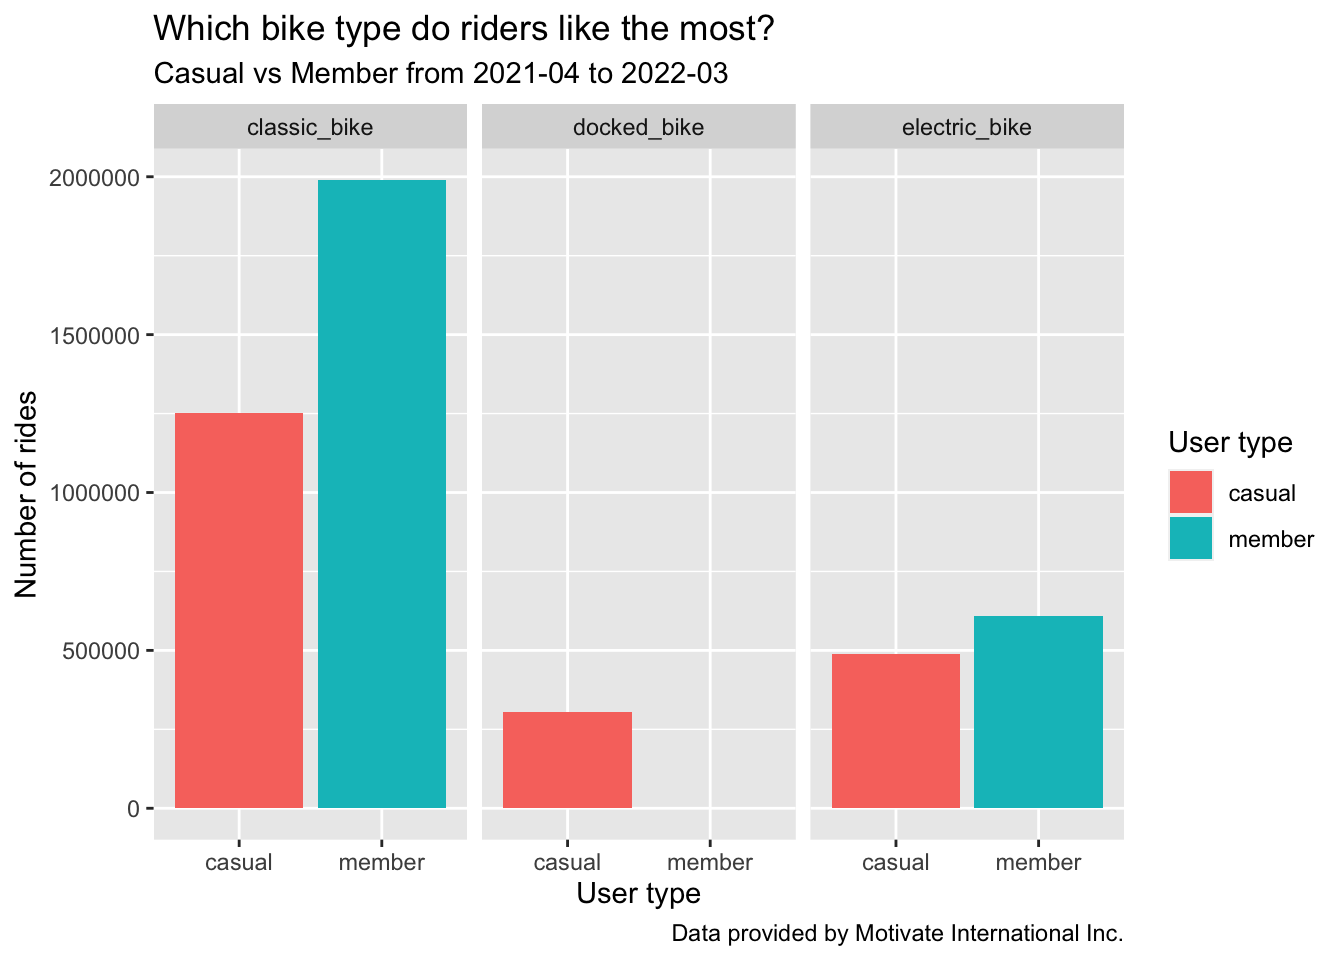
\includegraphics{capstone_bike_sharing_v02_files/figure-latex/unnamed-chunk-10-1.pdf}

\begin{Shaded}
\begin{Highlighting}[]
\NormalTok{trip\_data\_clean }\SpecialCharTok{\%\textgreater{}\%} \FunctionTok{group\_by}\NormalTok{(member\_casual,rideable\_type) }\SpecialCharTok{\%\textgreater{}\%} \FunctionTok{summarise}\NormalTok{(}\AttributeTok{count=}\FunctionTok{length}\NormalTok{(ride\_id),}\StringTok{"\%"}\OtherTok{=}\FunctionTok{length}\NormalTok{(ride\_id)}\SpecialCharTok{/}\FunctionTok{nrow}\NormalTok{(trip\_data\_clean)}\SpecialCharTok{*}\DecValTok{100}\NormalTok{) }\SpecialCharTok{\%\textgreater{}\%} \FunctionTok{arrange}\NormalTok{(}\FunctionTok{desc}\NormalTok{(count))}
\end{Highlighting}
\end{Shaded}

\begin{verbatim}
## `summarise()` has grouped output by 'member_casual'. You can override using the
## `.groups` argument.
\end{verbatim}

\begin{verbatim}
## # A tibble: 5 x 4
## # Groups:   member_casual [2]
##   member_casual rideable_type   count   `%`
##   <chr>         <chr>           <int> <dbl>
## 1 member        classic_bike  1989279 42.9 
## 2 casual        classic_bike  1252558 27.0 
## 3 member        electric_bike  607653 13.1 
## 4 casual        electric_bike  488183 10.5 
## 5 casual        docked_bike    303515  6.54
\end{verbatim}

\emph{Findings:} 1) Classic bikes are the most popular bike type for
both members and the casual. 2) Docked bikes are the least popular ones
and interestingly, docked bikes are only taken by the casual. More data
regarding different pricing plans for each type of bike and financial
aspect of the analysis are needed to find out why.

\begin{enumerate}
\def\labelenumi{\arabic{enumi}.}
\setcounter{enumi}{2}
\tightlist
\item
  How so riders behave differently each of the week?
\end{enumerate}

\begin{Shaded}
\begin{Highlighting}[]
\FunctionTok{ggplot}\NormalTok{(}\AttributeTok{data =}\NormalTok{ trip\_data\_clean)}\SpecialCharTok{+}\FunctionTok{geom\_bar}\NormalTok{(}\AttributeTok{position =} \StringTok{"dodge"}\NormalTok{,}\AttributeTok{mapping =} \FunctionTok{aes}\NormalTok{(}\AttributeTok{x=}\FunctionTok{factor}\NormalTok{(weekday, }\AttributeTok{level=}\FunctionTok{c}\NormalTok{(}\StringTok{\textquotesingle{}Monday\textquotesingle{}}\NormalTok{,}\StringTok{\textquotesingle{}Tuesday\textquotesingle{}}\NormalTok{,}\StringTok{\textquotesingle{}Wednesday\textquotesingle{}}\NormalTok{,}\StringTok{\textquotesingle{}Thursday\textquotesingle{}}\NormalTok{,}\StringTok{\textquotesingle{}Friday\textquotesingle{}}\NormalTok{,}\StringTok{\textquotesingle{}Saturday\textquotesingle{}}\NormalTok{,}\StringTok{\textquotesingle{}Sunday\textquotesingle{}}\NormalTok{)),}\AttributeTok{fill=}\NormalTok{member\_casual))}\SpecialCharTok{+}\FunctionTok{labs}\NormalTok{(}\AttributeTok{title=}\NormalTok{(}\StringTok{"How so riders behave differently each of the week?"}\NormalTok{),}\AttributeTok{subtitle =}\StringTok{"Casual vs Member from 2021{-}04 to 2022{-}03"}\NormalTok{, }\AttributeTok{x=}\StringTok{"User type"}\NormalTok{, }\AttributeTok{y=}\StringTok{"Number of rides"}\NormalTok{,}\AttributeTok{caption =} \StringTok{"1e+06=1,000,000, Data provided by Motivate International Inc."}\NormalTok{)}\SpecialCharTok{+}\FunctionTok{scale\_fill\_discrete}\NormalTok{(}\AttributeTok{name=}\StringTok{"User type"}\NormalTok{)}
\end{Highlighting}
\end{Shaded}

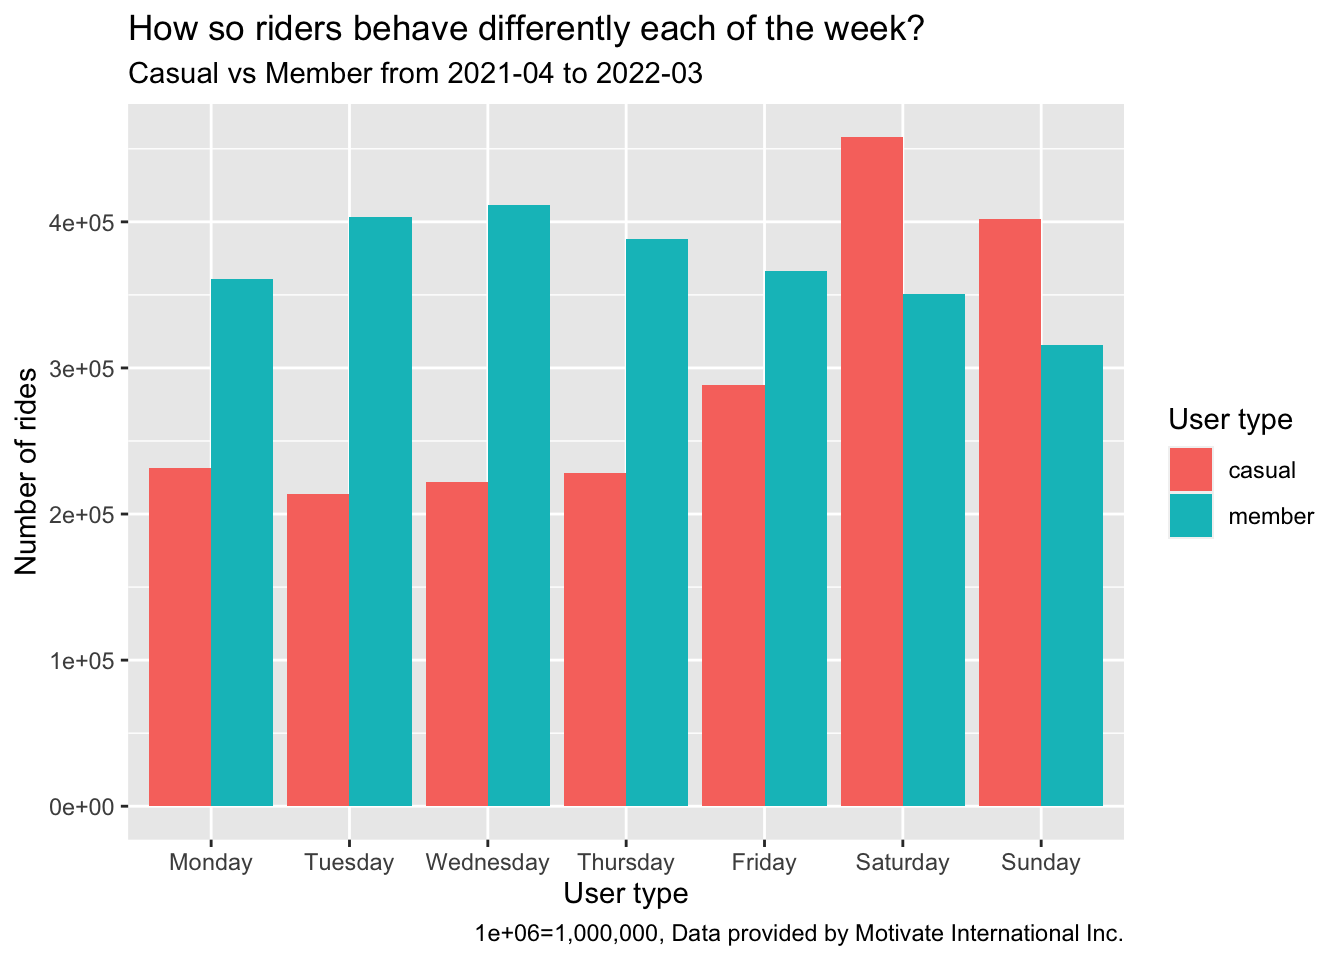
\includegraphics{capstone_bike_sharing_v02_files/figure-latex/unnamed-chunk-12-1.pdf}

\begin{Shaded}
\begin{Highlighting}[]
\NormalTok{trip\_data\_clean }\SpecialCharTok{\%\textgreater{}\%} \FunctionTok{group\_by}\NormalTok{(member\_casual,weekday) }\SpecialCharTok{\%\textgreater{}\%} \FunctionTok{summarise}\NormalTok{(}\AttributeTok{count=}\FunctionTok{length}\NormalTok{(ride\_id),}\StringTok{"\%"}\OtherTok{=}\FunctionTok{length}\NormalTok{(ride\_id)}\SpecialCharTok{/}\FunctionTok{nrow}\NormalTok{(trip\_data\_clean)}\SpecialCharTok{*}\DecValTok{100}\NormalTok{) }\SpecialCharTok{\%\textgreater{}\%} \FunctionTok{arrange}\NormalTok{(}\FunctionTok{desc}\NormalTok{(count))}
\end{Highlighting}
\end{Shaded}

\begin{verbatim}
## `summarise()` has grouped output by 'member_casual'. You can override using the
## `.groups` argument.
\end{verbatim}

\begin{verbatim}
## # A tibble: 14 x 4
## # Groups:   member_casual [2]
##    member_casual weekday    count   `%`
##    <chr>         <chr>      <int> <dbl>
##  1 casual        Saturday  458032  9.87
##  2 member        Wednesday 411738  8.87
##  3 member        Tuesday   403205  8.69
##  4 casual        Sunday    402105  8.66
##  5 member        Thursday  388455  8.37
##  6 member        Friday    366695  7.90
##  7 member        Monday    360579  7.77
##  8 member        Saturday  350489  7.55
##  9 member        Sunday    315771  6.80
## 10 casual        Friday    288223  6.21
## 11 casual        Monday    231686  4.99
## 12 casual        Thursday  228205  4.92
## 13 casual        Wednesday 222069  4.78
## 14 casual        Tuesday   213936  4.61
\end{verbatim}

\emph{Findings:} 1) Members mostly use bikes during week days and their
usage is relatively more consistent. Members use bikes less often on
weekends. 2) The casual use bikes mostly on weekends and you start to
notice increase in usage from Friday. They use bikes much less
frequently but consistent on the other week days (Monday, Tuesday,
Wednesday, Thursday). 3) On week days, members use more bikes than the
casual while on weekends, the casual use more bikes than members.

\begin{enumerate}
\def\labelenumi{\arabic{enumi}.}
\setcounter{enumi}{3}
\tightlist
\item
  How do riders behave differently across all hours of each day of the
  week?
\end{enumerate}

\begin{Shaded}
\begin{Highlighting}[]
\FunctionTok{ggplot}\NormalTok{(}\AttributeTok{data =}\NormalTok{ trip\_data\_clean)}\SpecialCharTok{+}\FunctionTok{geom\_bar}\NormalTok{(}\AttributeTok{mapping =} \FunctionTok{aes}\NormalTok{(}\AttributeTok{x=}\NormalTok{hour,}\AttributeTok{fill=}\NormalTok{member\_casual))}\SpecialCharTok{+}\FunctionTok{labs}\NormalTok{(}\AttributeTok{title=}\NormalTok{(}\StringTok{"How do riders behave differently across all hours of each day of the week?"}\NormalTok{),}\AttributeTok{subtitle =}\StringTok{"Casual vs Member from 2021{-}04 to 2022{-}03"}\NormalTok{, }\AttributeTok{x=}\StringTok{"Hours of the day"}\NormalTok{, }\AttributeTok{y=}\StringTok{"Number of rides"}\NormalTok{,}\AttributeTok{caption =} \StringTok{"Data provided by Motivate International Inc."}\NormalTok{)}\SpecialCharTok{+}\FunctionTok{scale\_fill\_discrete}\NormalTok{(}\AttributeTok{name=}\StringTok{"User type"}\NormalTok{)}\SpecialCharTok{+}\FunctionTok{facet\_wrap}\NormalTok{(}\FunctionTok{factor}\NormalTok{(weekday,}\AttributeTok{levels =} \FunctionTok{c}\NormalTok{(}\StringTok{\textquotesingle{}Monday\textquotesingle{}}\NormalTok{,}\StringTok{\textquotesingle{}Tuesday\textquotesingle{}}\NormalTok{,}\StringTok{\textquotesingle{}Wednesday\textquotesingle{}}\NormalTok{,}\StringTok{\textquotesingle{}Thursday\textquotesingle{}}\NormalTok{, }\StringTok{\textquotesingle{}Friday\textquotesingle{}}\NormalTok{,}\StringTok{\textquotesingle{}Saturday\textquotesingle{}}\NormalTok{,}\StringTok{\textquotesingle{}Sunday\textquotesingle{}}\NormalTok{))}\SpecialCharTok{\textasciitilde{}}\NormalTok{.)}\SpecialCharTok{+}\FunctionTok{theme}\NormalTok{(}\AttributeTok{axis.text.x =} \FunctionTok{element\_text}\NormalTok{(}\AttributeTok{angle =} \DecValTok{90}\NormalTok{,}\AttributeTok{size =} \DecValTok{7}\NormalTok{,))}
\end{Highlighting}
\end{Shaded}

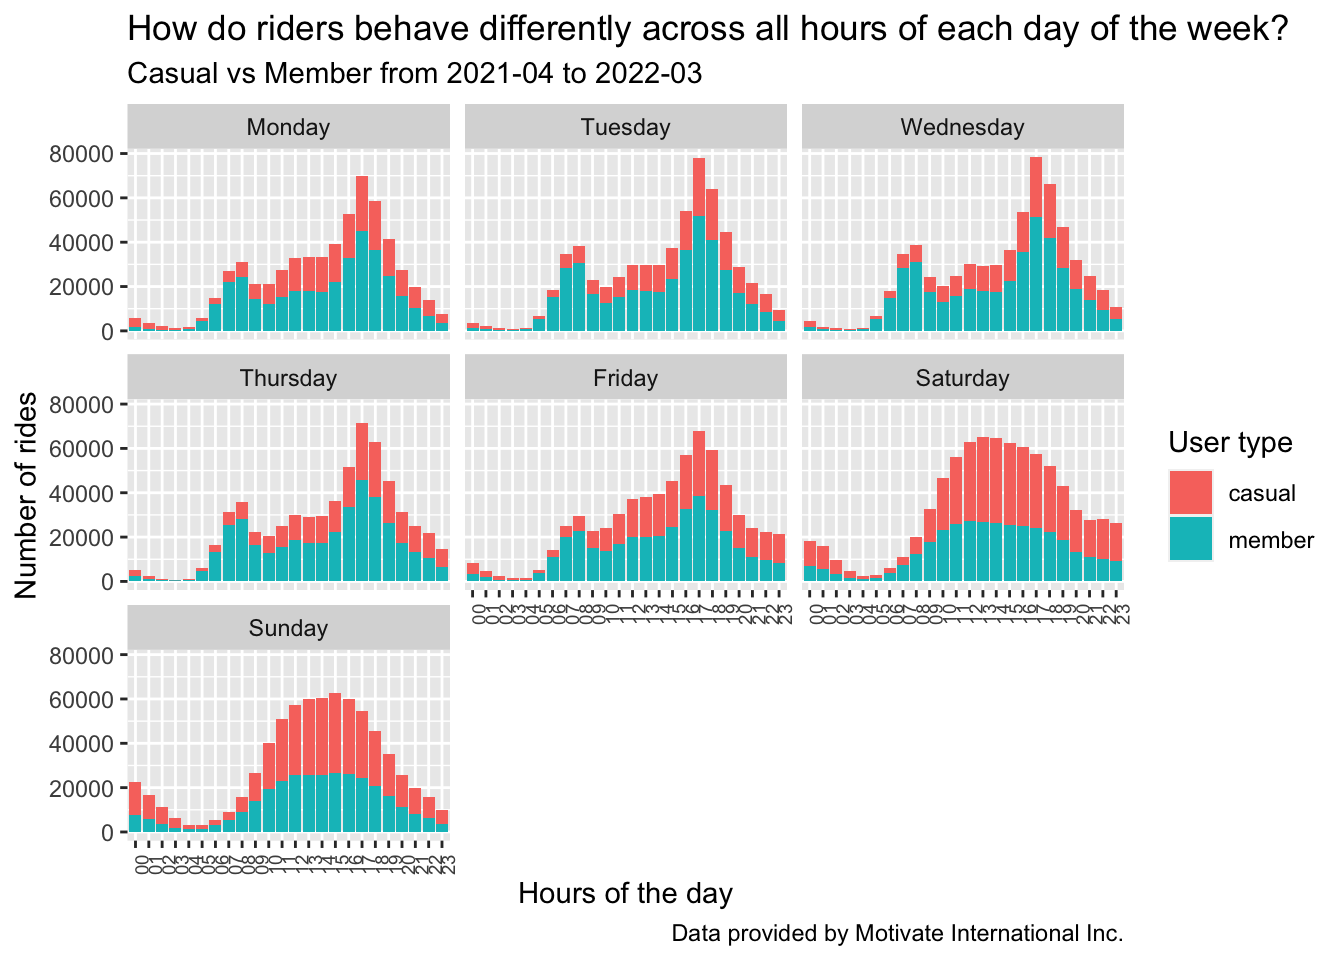
\includegraphics{capstone_bike_sharing_v02_files/figure-latex/unnamed-chunk-14-1.pdf}

\begin{Shaded}
\begin{Highlighting}[]
\NormalTok{trip\_data\_clean }\SpecialCharTok{\%\textgreater{}\%} \FunctionTok{group\_by}\NormalTok{(member\_casual,hour) }\SpecialCharTok{\%\textgreater{}\%} \FunctionTok{summarise}\NormalTok{(}\AttributeTok{count=}\FunctionTok{length}\NormalTok{(ride\_id),}\StringTok{"\%"}\OtherTok{=}\FunctionTok{length}\NormalTok{(ride\_id)}\SpecialCharTok{/}\FunctionTok{nrow}\NormalTok{(trip\_data\_clean)}\SpecialCharTok{*}\DecValTok{100}\NormalTok{) }\SpecialCharTok{\%\textgreater{}\%} \FunctionTok{arrange}\NormalTok{(}\FunctionTok{desc}\NormalTok{(hour))}
\end{Highlighting}
\end{Shaded}

\begin{verbatim}
## `summarise()` has grouped output by 'member_casual'. You can override using the
## `.groups` argument.
\end{verbatim}

\begin{verbatim}
## # A tibble: 48 x 4
## # Groups:   member_casual [2]
##    member_casual hour   count   `%`
##    <chr>         <chr>  <int> <dbl>
##  1 casual        23     58820 1.27 
##  2 member        23     40777 0.879
##  3 casual        22     76629 1.65 
##  4 member        22     60496 1.30 
##  5 casual        21     82936 1.79 
##  6 member        21     80117 1.73 
##  7 casual        20     97924 2.11 
##  8 member        20    108920 2.35 
##  9 casual        19    135346 2.92 
## 10 member        19    164261 3.54 
## # ... with 38 more rows
\end{verbatim}

\emph{Findings:} 1) On week days, both members and the casual have very
similar behavior pattern, where number of rides reaches its first peak
of the day at 8am, then goes down a bit from 9am to 10am, then starts
rising from 11am till its new peak of the day around 5pm. 2. On
weekends, number of riders don't reach its normal week day level till 9
or 10, then keeps rising and stays at relatively high level till 18pm or
19pm.

\begin{enumerate}
\def\labelenumi{\arabic{enumi}.}
\setcounter{enumi}{4}
\tightlist
\item
  How do riders behave differently across quarters?
\end{enumerate}

\begin{Shaded}
\begin{Highlighting}[]
\FunctionTok{ggplot}\NormalTok{(}\AttributeTok{data =}\NormalTok{ trip\_data\_clean)}\SpecialCharTok{+}\FunctionTok{geom\_bar}\NormalTok{(}\AttributeTok{position=}\StringTok{"dodge"}\NormalTok{,}\AttributeTok{mapping =} \FunctionTok{aes}\NormalTok{(}\AttributeTok{x=}\NormalTok{quarter,}\AttributeTok{fill=}\NormalTok{member\_casual))}\SpecialCharTok{+}\FunctionTok{labs}\NormalTok{(}\AttributeTok{title=}\NormalTok{(}\StringTok{"How do riders behave differently across quarters?"}\NormalTok{),}\AttributeTok{subtitle =}\StringTok{"Casual vs Member"}\NormalTok{, }\AttributeTok{x=}\StringTok{"User type"}\NormalTok{, }\AttributeTok{y=}\StringTok{"Number of rides"}\NormalTok{,}\AttributeTok{legend=}\StringTok{"User type"}\NormalTok{)}\SpecialCharTok{+}\FunctionTok{scale\_fill\_discrete}\NormalTok{(}\AttributeTok{name=}\StringTok{"User type"}\NormalTok{)}
\end{Highlighting}
\end{Shaded}

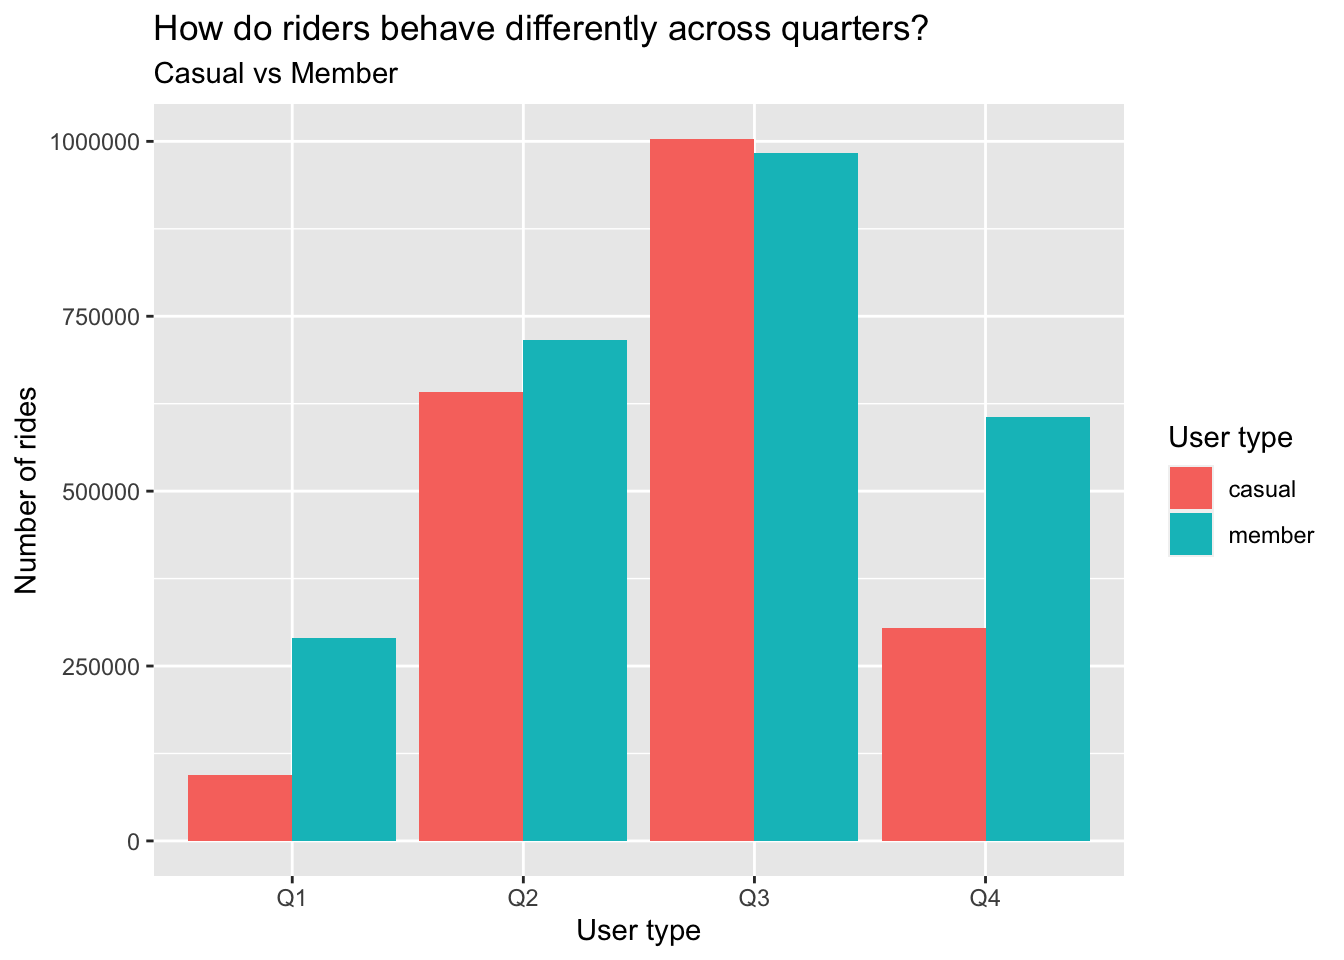
\includegraphics{capstone_bike_sharing_v02_files/figure-latex/unnamed-chunk-16-1.pdf}

\emph{Findings:} 1) Rides peaked in Q3 and valleyed in Q1 for both
members and the casual.

\begin{Shaded}
\begin{Highlighting}[]
\FunctionTok{ggplot}\NormalTok{(}\AttributeTok{data =}\NormalTok{ trip\_data\_clean)}\SpecialCharTok{+}\FunctionTok{geom\_bar}\NormalTok{(}\AttributeTok{position=}\StringTok{"dodge"}\NormalTok{,}\AttributeTok{mapping =} \FunctionTok{aes}\NormalTok{(}\AttributeTok{x=}\FunctionTok{factor}\NormalTok{(month,}\AttributeTok{levels =}\NormalTok{ (}\FunctionTok{c}\NormalTok{(}\StringTok{\textquotesingle{}January\textquotesingle{}}\NormalTok{,}\StringTok{\textquotesingle{}February\textquotesingle{}}\NormalTok{,}\StringTok{\textquotesingle{}March\textquotesingle{}}\NormalTok{,}\StringTok{\textquotesingle{}April\textquotesingle{}}\NormalTok{,}\StringTok{\textquotesingle{}May\textquotesingle{}}\NormalTok{,}\StringTok{\textquotesingle{}June\textquotesingle{}}\NormalTok{,}\StringTok{\textquotesingle{}July\textquotesingle{}}\NormalTok{,}\StringTok{\textquotesingle{}August\textquotesingle{}}\NormalTok{,}\StringTok{\textquotesingle{}September\textquotesingle{}}\NormalTok{,}\StringTok{\textquotesingle{}October\textquotesingle{}}\NormalTok{,}\StringTok{\textquotesingle{}November\textquotesingle{}}\NormalTok{,}\StringTok{\textquotesingle{}December\textquotesingle{}}\NormalTok{))),}\AttributeTok{fill=}\NormalTok{member\_casual))}\SpecialCharTok{+}\FunctionTok{labs}\NormalTok{(}\AttributeTok{title=}\NormalTok{(}\StringTok{"How do riders behave differently across all months of the year?"}\NormalTok{),}\AttributeTok{subtitle =}\StringTok{"Casual vs Member"}\NormalTok{, }\AttributeTok{x=}\StringTok{"User type"}\NormalTok{, }\AttributeTok{y=}\StringTok{"Number of rides"}\NormalTok{,}\AttributeTok{legend=}\StringTok{"User type"}\NormalTok{)}\SpecialCharTok{+}\FunctionTok{scale\_fill\_discrete}\NormalTok{(}\AttributeTok{name=}\StringTok{"User type"}\NormalTok{)}\SpecialCharTok{+}\FunctionTok{theme}\NormalTok{(}\AttributeTok{axis.text.x =} \FunctionTok{element\_text}\NormalTok{(}\AttributeTok{angle =} \DecValTok{45}\NormalTok{))}
\end{Highlighting}
\end{Shaded}

\includegraphics{capstone_bike_sharing_v02_files/figure-latex/unnamed-chunk-17-1.pdf}

\emph{Findings:} 1)

\hypertarget{where-do-riders-start-their-rides-and-where-do-they-go}{%
\subsubsection{Where do riders start their rides and where do they
go?}\label{where-do-riders-start-their-rides-and-where-do-they-go}}

First, let's get the map of Chicago. To decide the `bbox' values, I go
to \href{http://www.openstreetmap.org}{openstreetmap}

\begin{Shaded}
\begin{Highlighting}[]
\FunctionTok{library}\NormalTok{(ggplot2)}
\FunctionTok{library}\NormalTok{(maps)}
\end{Highlighting}
\end{Shaded}

\begin{verbatim}
## 
## Attaching package: 'maps'
\end{verbatim}

\begin{verbatim}
## The following object is masked from 'package:purrr':
## 
##     map
\end{verbatim}

\begin{Shaded}
\begin{Highlighting}[]
\FunctionTok{install.packages}\NormalTok{(}\StringTok{"ggmap"}\NormalTok{)}
\end{Highlighting}
\end{Shaded}

\begin{verbatim}
## Installing ggmap [3.0.0] ...
##  OK [linked cache]
\end{verbatim}

\begin{Shaded}
\begin{Highlighting}[]
\FunctionTok{library}\NormalTok{(ggmap)}
\end{Highlighting}
\end{Shaded}

\begin{verbatim}
## Google's Terms of Service: https://cloud.google.com/maps-platform/terms/.
\end{verbatim}

\begin{verbatim}
## Please cite ggmap if you use it! See citation("ggmap") for details.
\end{verbatim}

\begin{Shaded}
\begin{Highlighting}[]
\NormalTok{map\_chicago}\OtherTok{\textless{}{-}}\FunctionTok{get\_stamenmap}\NormalTok{(}\AttributeTok{bbox =} \FunctionTok{c}\NormalTok{(}\AttributeTok{left=}\SpecialCharTok{{-}}\FloatTok{88.3}\NormalTok{, }\AttributeTok{bottom=}\FloatTok{41.3}\NormalTok{, }\AttributeTok{right=}\SpecialCharTok{{-}}\FloatTok{87.0}\NormalTok{, }\AttributeTok{top=}\FloatTok{42.4}\NormalTok{), }\AttributeTok{maptype=}\StringTok{"terrain"}\NormalTok{,}\AttributeTok{zoom =} \DecValTok{11}\NormalTok{)}
\end{Highlighting}
\end{Shaded}

\begin{verbatim}
## 81 tiles needed, this may take a while (try a smaller zoom).
\end{verbatim}

\begin{verbatim}
## Source : http://tile.stamen.com/terrain/11/521/757.png
\end{verbatim}

\begin{verbatim}
## Source : http://tile.stamen.com/terrain/11/522/757.png
\end{verbatim}

\begin{verbatim}
## Source : http://tile.stamen.com/terrain/11/523/757.png
\end{verbatim}

\begin{verbatim}
## Source : http://tile.stamen.com/terrain/11/524/757.png
\end{verbatim}

\begin{verbatim}
## Source : http://tile.stamen.com/terrain/11/525/757.png
\end{verbatim}

\begin{verbatim}
## Source : http://tile.stamen.com/terrain/11/526/757.png
\end{verbatim}

\begin{verbatim}
## Source : http://tile.stamen.com/terrain/11/527/757.png
\end{verbatim}

\begin{verbatim}
## Source : http://tile.stamen.com/terrain/11/528/757.png
\end{verbatim}

\begin{verbatim}
## Source : http://tile.stamen.com/terrain/11/529/757.png
\end{verbatim}

\begin{verbatim}
## Source : http://tile.stamen.com/terrain/11/521/758.png
\end{verbatim}

\begin{verbatim}
## Source : http://tile.stamen.com/terrain/11/522/758.png
\end{verbatim}

\begin{verbatim}
## Source : http://tile.stamen.com/terrain/11/523/758.png
\end{verbatim}

\begin{verbatim}
## Source : http://tile.stamen.com/terrain/11/524/758.png
\end{verbatim}

\begin{verbatim}
## Source : http://tile.stamen.com/terrain/11/525/758.png
\end{verbatim}

\begin{verbatim}
## Source : http://tile.stamen.com/terrain/11/526/758.png
\end{verbatim}

\begin{verbatim}
## Source : http://tile.stamen.com/terrain/11/527/758.png
\end{verbatim}

\begin{verbatim}
## Source : http://tile.stamen.com/terrain/11/528/758.png
\end{verbatim}

\begin{verbatim}
## Source : http://tile.stamen.com/terrain/11/529/758.png
\end{verbatim}

\begin{verbatim}
## Source : http://tile.stamen.com/terrain/11/521/759.png
\end{verbatim}

\begin{verbatim}
## Source : http://tile.stamen.com/terrain/11/522/759.png
\end{verbatim}

\begin{verbatim}
## Source : http://tile.stamen.com/terrain/11/523/759.png
\end{verbatim}

\begin{verbatim}
## Source : http://tile.stamen.com/terrain/11/524/759.png
\end{verbatim}

\begin{verbatim}
## Source : http://tile.stamen.com/terrain/11/525/759.png
\end{verbatim}

\begin{verbatim}
## Source : http://tile.stamen.com/terrain/11/526/759.png
\end{verbatim}

\begin{verbatim}
## Source : http://tile.stamen.com/terrain/11/527/759.png
\end{verbatim}

\begin{verbatim}
## Source : http://tile.stamen.com/terrain/11/528/759.png
\end{verbatim}

\begin{verbatim}
## Source : http://tile.stamen.com/terrain/11/529/759.png
\end{verbatim}

\begin{verbatim}
## Source : http://tile.stamen.com/terrain/11/521/760.png
\end{verbatim}

\begin{verbatim}
## Source : http://tile.stamen.com/terrain/11/522/760.png
\end{verbatim}

\begin{verbatim}
## Source : http://tile.stamen.com/terrain/11/523/760.png
\end{verbatim}

\begin{verbatim}
## Source : http://tile.stamen.com/terrain/11/524/760.png
\end{verbatim}

\begin{verbatim}
## Source : http://tile.stamen.com/terrain/11/525/760.png
\end{verbatim}

\begin{verbatim}
## Source : http://tile.stamen.com/terrain/11/526/760.png
\end{verbatim}

\begin{verbatim}
## Source : http://tile.stamen.com/terrain/11/527/760.png
\end{verbatim}

\begin{verbatim}
## Source : http://tile.stamen.com/terrain/11/528/760.png
\end{verbatim}

\begin{verbatim}
## Source : http://tile.stamen.com/terrain/11/529/760.png
\end{verbatim}

\begin{verbatim}
## Source : http://tile.stamen.com/terrain/11/521/761.png
\end{verbatim}

\begin{verbatim}
## Source : http://tile.stamen.com/terrain/11/522/761.png
\end{verbatim}

\begin{verbatim}
## Source : http://tile.stamen.com/terrain/11/523/761.png
\end{verbatim}

\begin{verbatim}
## Source : http://tile.stamen.com/terrain/11/524/761.png
\end{verbatim}

\begin{verbatim}
## Source : http://tile.stamen.com/terrain/11/525/761.png
\end{verbatim}

\begin{verbatim}
## Source : http://tile.stamen.com/terrain/11/526/761.png
\end{verbatim}

\begin{verbatim}
## Source : http://tile.stamen.com/terrain/11/527/761.png
\end{verbatim}

\begin{verbatim}
## Source : http://tile.stamen.com/terrain/11/528/761.png
\end{verbatim}

\begin{verbatim}
## Source : http://tile.stamen.com/terrain/11/529/761.png
\end{verbatim}

\begin{verbatim}
## Source : http://tile.stamen.com/terrain/11/521/762.png
\end{verbatim}

\begin{verbatim}
## Source : http://tile.stamen.com/terrain/11/522/762.png
\end{verbatim}

\begin{verbatim}
## Source : http://tile.stamen.com/terrain/11/523/762.png
\end{verbatim}

\begin{verbatim}
## Source : http://tile.stamen.com/terrain/11/524/762.png
\end{verbatim}

\begin{verbatim}
## Source : http://tile.stamen.com/terrain/11/525/762.png
\end{verbatim}

\begin{verbatim}
## Source : http://tile.stamen.com/terrain/11/526/762.png
\end{verbatim}

\begin{verbatim}
## Source : http://tile.stamen.com/terrain/11/527/762.png
\end{verbatim}

\begin{verbatim}
## Source : http://tile.stamen.com/terrain/11/528/762.png
\end{verbatim}

\begin{verbatim}
## Source : http://tile.stamen.com/terrain/11/529/762.png
\end{verbatim}

\begin{verbatim}
## Source : http://tile.stamen.com/terrain/11/521/763.png
\end{verbatim}

\begin{verbatim}
## Source : http://tile.stamen.com/terrain/11/522/763.png
\end{verbatim}

\begin{verbatim}
## Source : http://tile.stamen.com/terrain/11/523/763.png
\end{verbatim}

\begin{verbatim}
## Source : http://tile.stamen.com/terrain/11/524/763.png
\end{verbatim}

\begin{verbatim}
## Source : http://tile.stamen.com/terrain/11/525/763.png
\end{verbatim}

\begin{verbatim}
## Source : http://tile.stamen.com/terrain/11/526/763.png
\end{verbatim}

\begin{verbatim}
## Source : http://tile.stamen.com/terrain/11/527/763.png
\end{verbatim}

\begin{verbatim}
## Source : http://tile.stamen.com/terrain/11/528/763.png
\end{verbatim}

\begin{verbatim}
## Source : http://tile.stamen.com/terrain/11/529/763.png
\end{verbatim}

\begin{verbatim}
## Source : http://tile.stamen.com/terrain/11/521/764.png
\end{verbatim}

\begin{verbatim}
## Source : http://tile.stamen.com/terrain/11/522/764.png
\end{verbatim}

\begin{verbatim}
## Source : http://tile.stamen.com/terrain/11/523/764.png
\end{verbatim}

\begin{verbatim}
## Source : http://tile.stamen.com/terrain/11/524/764.png
\end{verbatim}

\begin{verbatim}
## Source : http://tile.stamen.com/terrain/11/525/764.png
\end{verbatim}

\begin{verbatim}
## Source : http://tile.stamen.com/terrain/11/526/764.png
\end{verbatim}

\begin{verbatim}
## Source : http://tile.stamen.com/terrain/11/527/764.png
\end{verbatim}

\begin{verbatim}
## Source : http://tile.stamen.com/terrain/11/528/764.png
\end{verbatim}

\begin{verbatim}
## Source : http://tile.stamen.com/terrain/11/529/764.png
\end{verbatim}

\begin{verbatim}
## Source : http://tile.stamen.com/terrain/11/521/765.png
\end{verbatim}

\begin{verbatim}
## Source : http://tile.stamen.com/terrain/11/522/765.png
\end{verbatim}

\begin{verbatim}
## Source : http://tile.stamen.com/terrain/11/523/765.png
\end{verbatim}

\begin{verbatim}
## Source : http://tile.stamen.com/terrain/11/524/765.png
\end{verbatim}

\begin{verbatim}
## Source : http://tile.stamen.com/terrain/11/525/765.png
\end{verbatim}

\begin{verbatim}
## Source : http://tile.stamen.com/terrain/11/526/765.png
\end{verbatim}

\begin{verbatim}
## Source : http://tile.stamen.com/terrain/11/527/765.png
\end{verbatim}

\begin{verbatim}
## Source : http://tile.stamen.com/terrain/11/528/765.png
\end{verbatim}

\begin{verbatim}
## Source : http://tile.stamen.com/terrain/11/529/765.png
\end{verbatim}

\begin{Shaded}
\begin{Highlighting}[]
\FunctionTok{ggmap}\NormalTok{(map\_chicago)}
\end{Highlighting}
\end{Shaded}

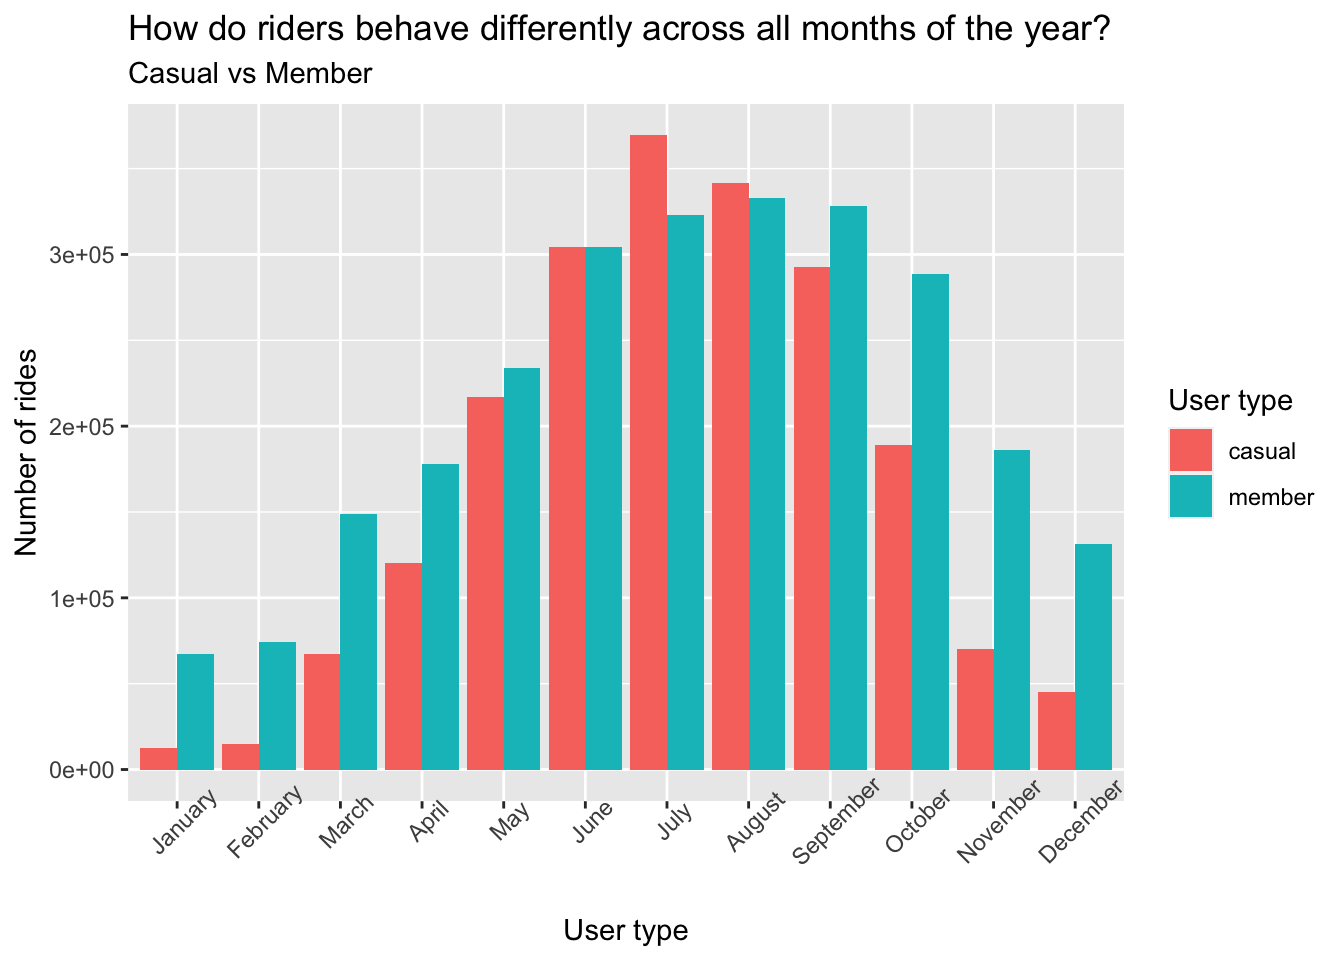
\includegraphics{capstone_bike_sharing_v02_files/figure-latex/unnamed-chunk-18-1.pdf}

Second, plot starting points and ending points on the map of Chicago

\begin{Shaded}
\begin{Highlighting}[]
\FunctionTok{ggmap}\NormalTok{(map\_chicago)}\SpecialCharTok{+}\FunctionTok{geom\_jitter}\NormalTok{(trip\_data\_clean,}\AttributeTok{mapping =} \FunctionTok{aes}\NormalTok{(}\AttributeTok{x=}\NormalTok{start\_lng,}\AttributeTok{y=}\NormalTok{start\_lat),}\AttributeTok{color=}\StringTok{"yellow"}\NormalTok{)}\SpecialCharTok{+}\FunctionTok{facet\_wrap}\NormalTok{(}\SpecialCharTok{\textasciitilde{}}\NormalTok{member\_casual)}\SpecialCharTok{+}\FunctionTok{labs}\NormalTok{(}\AttributeTok{title =} \StringTok{"Where do riders start their rides?"}\NormalTok{,}\AttributeTok{subtitle =} \StringTok{"Casual vs Member from 2021{-}04 to 2022{-}03"}\NormalTok{, }\AttributeTok{x=}\StringTok{"Lng"}\NormalTok{, }\AttributeTok{y=}\StringTok{" Lat"}\NormalTok{)}\SpecialCharTok{+}\FunctionTok{scale\_fill\_discrete}\NormalTok{(}\AttributeTok{name=}\StringTok{"starting points"}\NormalTok{)}\SpecialCharTok{+}\FunctionTok{theme}\NormalTok{(}\AttributeTok{axis.text.x =} \FunctionTok{element\_text}\NormalTok{(}\AttributeTok{angle =} \DecValTok{90}\NormalTok{))}
\end{Highlighting}
\end{Shaded}

\begin{verbatim}
## Warning: Removed 1 rows containing missing values (geom_point).
\end{verbatim}

\includegraphics{capstone_bike_sharing_v02_files/figure-latex/unnamed-chunk-19-1.pdf}

\begin{Shaded}
\begin{Highlighting}[]
\FunctionTok{ggmap}\NormalTok{(map\_chicago)}\SpecialCharTok{+}\FunctionTok{geom\_jitter}\NormalTok{(trip\_data\_clean,}\AttributeTok{mapping =} \FunctionTok{aes}\NormalTok{(}\AttributeTok{x=}\NormalTok{end\_lng,}\AttributeTok{y=}\NormalTok{end\_lat),}\AttributeTok{color=}\StringTok{"red"}\NormalTok{)}\SpecialCharTok{+}\FunctionTok{facet\_wrap}\NormalTok{(}\SpecialCharTok{\textasciitilde{}}\NormalTok{member\_casual)}\SpecialCharTok{+}\FunctionTok{labs}\NormalTok{(}\AttributeTok{title =} \StringTok{"Where do riders go with their rides?"}\NormalTok{,}\AttributeTok{subtitle =} \StringTok{"Casual vs Member from 2021{-}04 to 2022{-}03"}\NormalTok{, }\AttributeTok{x=}\StringTok{"Lng"}\NormalTok{, }\AttributeTok{y=}\StringTok{" Lat"}\NormalTok{)}\SpecialCharTok{+}\FunctionTok{scale\_fill\_discrete}\NormalTok{(}\AttributeTok{name=}\StringTok{"ending points"}\NormalTok{)}\SpecialCharTok{+}\FunctionTok{theme}\NormalTok{(}\AttributeTok{axis.text.x =} \FunctionTok{element\_text}\NormalTok{(}\AttributeTok{angle =} \DecValTok{90}\NormalTok{))}
\end{Highlighting}
\end{Shaded}

\includegraphics{capstone_bike_sharing_v02_files/figure-latex/unnamed-chunk-19-2.pdf}
\emph{Findings:} 1) Members and the casual have very similar behavior
pattern in terms of where they start their rides and where they go with
rides. But occasionally, the casual are more likely \#\# A summary of
your analysis

\hypertarget{your-top-three-recommendations-based-on-your-analysis}{%
\subsection{Your top three recommendations based on your
analysis}\label{your-top-three-recommendations-based-on-your-analysis}}

\end{document}
